\documentclass[a4paper, 12pt]{article}%тип документа

%отступы
\usepackage[left=2cm,right=2cm,top=2cm,bottom=3cm,bindingoffset=0cm]{geometry}
\setlength{\parindent}{5ex}

%Русский язык
\usepackage[T2A]{fontenc} %кодировка
\usepackage[utf8]{inputenc} %кодировка исходного кода
\usepackage[english,russian]{babel} %локализация и переносы

%Вставка картинок
\usepackage{graphicx}
\graphicspath{{pictures/}}
\DeclareGraphicsExtensions{.pdf,.png,.jpg}

%Графики
\usepackage{pgfplots}
\pgfplotsset{compat=1.9}

%Математика
\usepackage{amsmath, amsfonts, amssymb, amsthm, mathtools}

%Таблицы
\usepackage{longtable} 
\usepackage{float}

%Римские цифры
\newcommand{\RomanNumeralCaps}[1]{\uppercase\expandafter{\romannumeral#1}}

\usepackage{multirow}


\begin{document}
	\begin{titlepage}
		\begin{center}
			\textsc{Федеральное государственное автономное образовательное учреждение высшего образования«Московский физико-технический институт (национальный исследовательский университет)»\\[5mm]
			}
			
			\vfill
			
			\textbf{Отчёт по лабораторной работы 3.1.3\\[3mm]
				Измерение магнитного поля Земли
				\\[50mm]
			}
			
		\end{center}
		
		\hfill
		\begin{minipage}{.5\textwidth}
			Выполнил студент:\\[2mm]
			Сериков Василий Романович\\[2mm]
			группа: Б03-102\\[5mm]
			
		\end{minipage}
		\vfill
		\begin{center}
			Москва, 2022 г.
		\end{center}
		
	\end{titlepage}
	
	\newpage
	\textbf{Аннотация}\\
	
	
	\textbf{Цель работы: }\\
	
	Исследовать свойства постоянных неодимовых магнитов;
	измерить с их помощью горизонтальную и вертикальную составляющие
	индукции магнитного поля Земли и магнитное наклонение.\\
	
	\textbf{В работе используются: }\\
	
	Неодимовые магниты; тонкая нить для изготовления крутильного маятника; медная проволока; электронные весы; секундомер; измеритель магнитной индукции; штангенциркуль; брусок, линейка
	и штатив из немагнитных материалов; набор гирь и разновесов.\\
	
	\textbf{Теоретические сведения: } \\
	
	Простейший магнитный диполь может быть образован витком с током или постоянным магнитом. По определению, магнитный момент $\overrightarrow{\mathfrak m }$ тонкого витка площадью $S$ с током $I$ равен
	$$
	\overrightarrow{\mathfrak m}=\dfrac{I}{c}\vec{S}=\dfrac{I}{c}S\vec{n},
	$$
	где $\vec{S}=S\vec{n}$ -- вектор площади круга контура. Если размеры контура с током или магнитной стрелки малы по сравнению расстоянием до диполя, то соответствующий магнитный диполь называют элементарным или точечным.\\
	Магнитное поле точечного диполя определяется по формуле, аналогичной формуле для поля
	элементарного электрического диполя:
	$$
	\vec{B}=\dfrac{3(\overrightarrow{\mathfrak m},\vec{r})\vec{r}}{r^5} - \dfrac{\overrightarrow{\mathfrak m}}{r^3}
	$$ 
	В магнитном поле с индукцией $B$
	на точечный магнитный диполь 
	действует механический
	момент сил:
	$$
	\vec{\mathcal M} = \overrightarrow{\mathfrak m}\times \vec{B}.
	$$
	Под действием вращающего момента $\vec{\mathcal M}$ виток с током или постоянный магнит поворачивается
	так, чтобы его магнитный момент выстроился вдоль вектора индукции магнитного поля. Это —
	положение устойчивого равновесия: при отклонении от этого положения возникает механический
	момент внешних сил, возвращающий диполь к положению равновесия. В положении, когда $\overrightarrow{\mathfrak m}$ и $\vec{B}$
	параллельны, но направлены противоположно друг другу, также имеет место равновесие ($\mathcal M$ = 0),
	но такое равновесие неустойчиво: малейшее отклонение от этого положения приведёт к появлению
	момента сил, стремящихся отклонить диполь ещё дальше от начального положения.\\
	Магнитный диполь в магнитном поле обладает энергией:
	$$
	W = -(\overrightarrow{\mathfrak m},\vec{B})
	$$
	В неоднородном поле на точечный магнитный диполь, кроме момента сил, действует ещё и сила:
	$$
	\vec{F}=(\overrightarrow{\mathfrak m},\vec{\triangledown})\vec{B}
	$$
	Используя формулы для момента силы, силы и энергии, не сложно выяснить, как ведёт себя
	свободный магнитный диполь в неоднородном магнитном поле: он выстраивается вдоль силовых
	линий магнитного поля и, кроме того, под действием результирующей силы, возникающей из-за
	неоднородности поля, втягивается в область более сильного магнитного поля, т.е. в область, где он
	обладает меньшей энергией.\\
	Зная магнитные моменты $\mathfrak {m_1} = \mathfrak {m_2}  = \mathfrak m$ двух небольших постоянных магнитов, можно рассчитать силу
	их взаимодействия:
	$$
	F = \mathfrak m \dfrac{\partial B}{\partial r}=-6\dfrac{\mathfrak m^2}{r^4}.
	$$
	
	\textbf{Экспериментальная установка: }\\
	
	В настоящей работе используются неодимовые магниты шарообразной формы.
	Для эксперимента важно, что: шары намагничены однородно, вещество, из которого изготовлены магниты, является магнитожёстким материалом.\\
	
	Магнитное поле однородно намагниченного шара радиусом R может
	быть вычислено точно. На расстояниях r$\geq$R от центра шара оно совпадает с полем точечного магнитного диполя, расположенного в центре, магнитный момент $\mathfrak m$ которого совпадает с полным моментом шара.
	Внутри шара магнитное поле однородно: условия непрерывности нормальной компоненты индукции на поверхности
	шара нетрудно получить, что при r < R
	$$
	B_0 = \frac{\mu_0 \mathfrak m}{2\pi R^3}
	$$
	
	Намагниченность(I) — характеристика вещества постоянных магнитов, определяющая, в
	частности, величину остаточной магнитной индукции $B_r = \mu_0 I$. Индукция магнитного поля $\overrightarrow{B_p}$
	на полюсах однородно намагниченного шара связана с величиной намагниченности и остаточной магнитной индукцией формулами
	$$
	{B_p}=B_0=\dfrac{2}{3}{B_r}.
	$$
	
\textbf{Определение величины магнитного момента магнитных шариков}\\

	\textbf{Метод А}\\
	
	Величину магнитного момента одинаковых шариков
	можно рассчитать, зная их массу $m$ и определив максимальное расстояние $r_{max}$, на котором они ещё удерживают друг
	друга в поле тяжести. При максимальном расстоянии сила тяжести шариков равна силе их магнитного притяжения:
	\begin{center}
		$\dfrac{6\mathfrak m^2}{r_{max}^4}=mg\Rightarrow$ {$\mathfrak m = \sqrt{\dfrac{mgr_{max}^4}{6}}$}
	\end{center}

	\textbf{Метод В}\\
	
	Если сила сцепления двух одинаковых шаров диаметром $d$ c магнитными моментами $\mathfrak m$ равна:
	$$
	F_0 = \dfrac{6\mathfrak m^2}{d^4}
	$$
	то минимальный вес цепочки, при которой она оторвётся от верхнего шарика равен: $F \approx 1.08 F_0$. Тогда\\
	\begin{center}
		{$\mathfrak m = \sqrt{\dfrac{Fd^4}{6.48}}$}
	\end{center}

	\textbf{Определение величины магнитного поля Земли}\\
	
	\textbf{Горизонтальная составляющая}\\

	Магнитная <<стрелка>> образована из $n$ сцепленных друг с другом противоположными полюсами шариков и с помощью $\Lambda$-образного подвеса подвешена в горизонтальном положении. При отклонении «стрелки» на угол $\theta$ от равновесного положения в горизонтальной плоскости возникают крутильные колебания вокруг вертикальной оси, проходящей через середину стрелки. При малых амплитудах уравнение колебаний
	стрелки имеет вид:
	$$
	I_n \dfrac{d^2 \theta}{dt^2} + P_0 B_h \theta = 0,
	$$ 
	где $P_0$ -- магнитный момент стрелки, $B_h$ -- горизонтальная составляющая магнитного поля Земли, $I_n \approx \dfrac{1}{12}n^3 m d^3$, тогда период колебаний $T = kn$, где $k = \pi \sqrt{\dfrac{md^2}{3\mathfrak m B_h}}$. Измеряя зависимость $T=T(n)$, находится $B_h$:
	\begin{center}
		{$B_h = \dfrac{\pi^2 m d^2}{3k^2 \mathfrak m}$}
	\end{center}
	\begin{figure}[h]
	\center{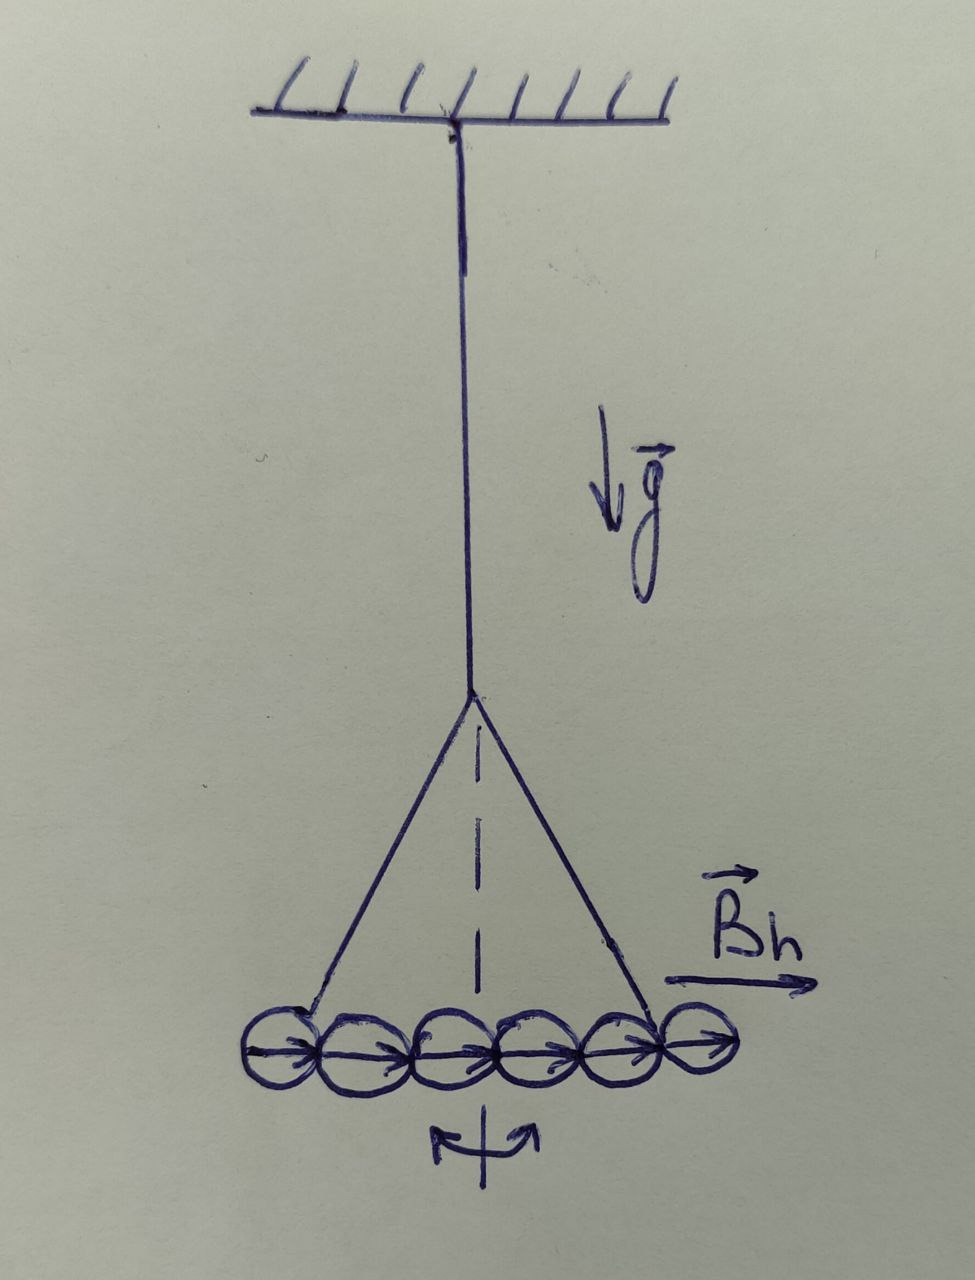
\includegraphics [scale=0.3]{photo1.jpeg}}
	\caption{Измерение горизонтальной составляющей поля и магнитного наклонения}
\end{figure}
	
	\textbf{Вертикальная составляющая} \\
	
	Магнитная «стрелка», составленная из чётного числа
	шариков и подвешенная на тонкой нити за середину, расположится не горизонтально, а под некоторым, отличным от нуля, углом к горизонту. Это связано с тем, что вектор $\vec{B}$ индукции магнитного поля Земли в общем случае не горизонтален, а образует с горизонтом
	угол $\beta$, зависящим от географической широты $\varphi$
	места, где проводится опыт. Величина угла $\beta$
	называется магнитным наклонением.\\
	С помощью небольшого дополнительного грузика «стрелку» можно «выровнять». Момент $\mathcal M$ силы тяжести уравновешивающего груза пропорционален числу $n$ шариков, образующих магнитную «стрелку» $\mathcal M(n) = n\mathfrak m B_v = m_{\text{гр}}g r_{\text{гр}}$, то есть
	\begin{center}
		{$B_v = \dfrac{ m_{\text{гр}}g r_{\text{гр}}}{\mathfrak m n}$}
	\end{center}
\begin{figure}[H]
	\center{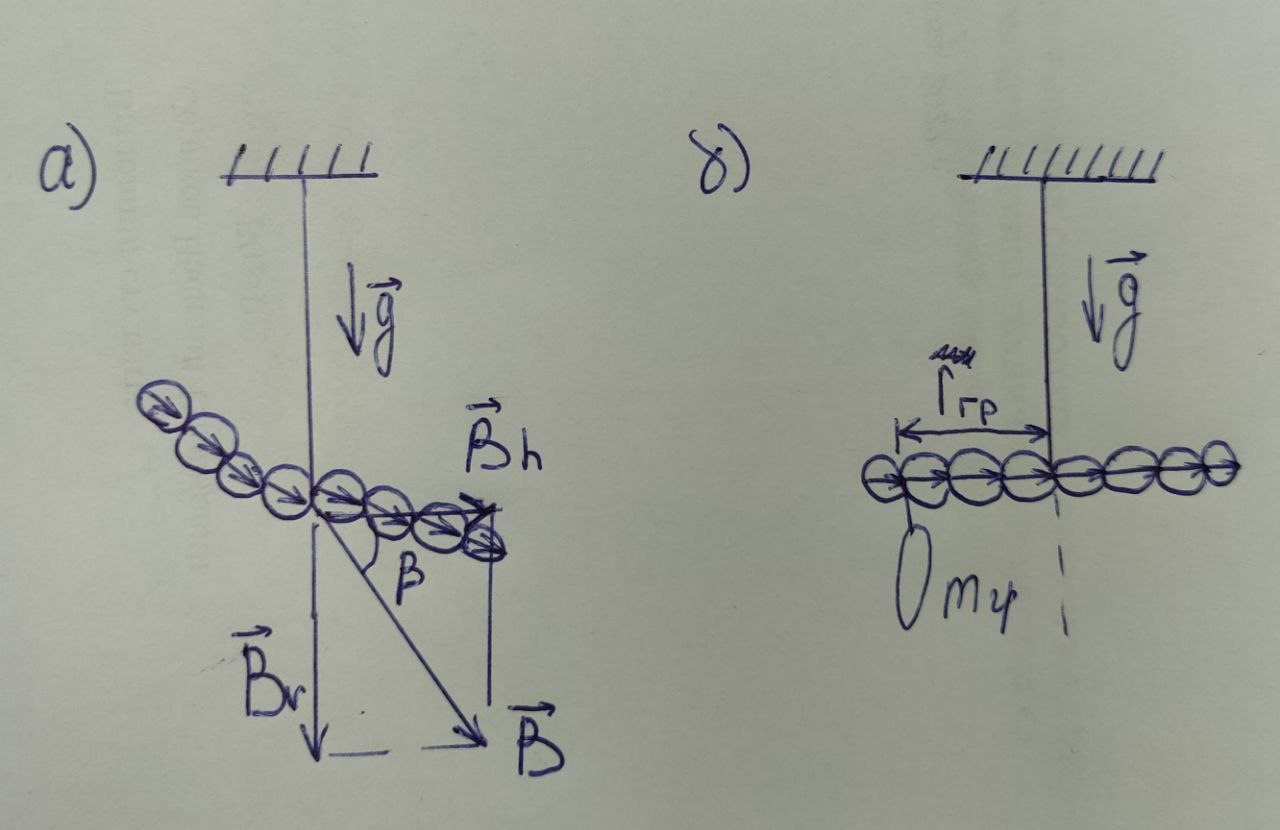
\includegraphics [scale=0.3]{photo2.jpeg}}
	\caption{Измерение вертикальной составляющей поля и магнитного наклонения}
\end{figure}


	\newpage
	
	\textbf{Ход работы и обработка результатов: }
	
	\begin{enumerate}
		
		\item Измерим массу шариков и их диаметр. Получим $m = 0,818 \pm 0,007$ г, $d = 6,39 \pm 0,01$ мм.
		
		\item С помощью магнетометра измерьте индукцию поля $B_p$ на полюсах шарика. Чтобы определить полюс шарика, соединим его с еще одним шариком, учтем влияние второго шарика и получим $B_p$. $B_p = B^{full} - B^{1ball} = 226,0 - 17,3 = 208,7 \pm 0,3$ мТл.
		
		\item Определим, на каком максимальном расстоянии $r_{max}$ шарики удерживают друг друга в поле тяжести Земли и рассчитаем величину магнитного момента магнитика $\mathfrak m$. $r_{max} = 23,0 $ мм, 
		
		$$ \mathfrak m = \sqrt{\dfrac{mgr_{max}^4}{6}} = 62 \pm 5 \text{  эрг/Гс}$$ 
		
		\item Рассчитаем силу сцепления двух шаров и по ней определим магнитный момент шарика $\mathfrak m$. $F_{max} = m_{max} g = 3,12$ Н.
		$$ \mathfrak m = \sqrt{\dfrac{Fd^4}{6.48}} = 89,8 \pm 0,3\text{  эрг/Гс}$$
		 
		
		\item Рассчитаем величину намагниченности материала шариков I и
		остаточную индукцию магнитного поля $B_r$. $I = \mathfrak m / V = 654 \pm 6$ эрг/(Гс$\cdot$см$^3$)
		
		$$ B_r = 4\pi I =  8218 \pm 80 \text{  Гс}$$
		$$ B_p = 2/3 \cdot B_r = 5478 \pm 53 \text{  Гс}$$
		
		\item Определим горизонтальную составляющую магнитного поля Землю с помощью крутильного маятника и магнитных шариков. Проведем серию измерений периодов крутильных колебаний для различного количества шариков. Полученные данные занесем в таблицу 1.
		
		\begin{longtable} {|c|c|c|c|c|c|c|c|}
			\hline
			n & 12 & 10 & 8 & 7 & 6 & 4 & 3    \\ \hline
			T, с & 4,9 & 3,9 & 2,9 & 2,7 & 2,2 & 2,0 & 1,2\\ \hline
			\caption{Периоды крутильных колебаний, $\sigma = 0,1 c$}
		\end{longtable}
		
		\item Определим вертикальную составляющую магнитного поля Земли.
		Для этого определим механический момент сил, действующий со стороны магнитного поля Земли на горизонтально расположенную магнитную «стрелку». Полученные данные занесем в таблицу 2.
		
		\begin{longtable} {|c|c|c|c|c|}
			\hline
			n &  10 & 8 & 6 & 4   \\ \hline
			$\mathcal M,$ дин$\cdot$см & 274 & 183 & 115 & 100 \\ \hline
			\caption{Моменты сил, действующие на стрелку, $\varepsilon = 1\% $}
		\end{longtable}
	
	\newpage
		
		
		\item Построим график зависимости T(n). По значению углового коэффициента рассчитаем величину горизонтальной составляющей магнитного поля Земли.
		
		$$ B_h = \dfrac{\pi^2 m d^2}{3k^2 \mathfrak m} = 0,086 \pm 0,004 \text{  Гс}$$
		
		\begin{figure}[H]
			\center{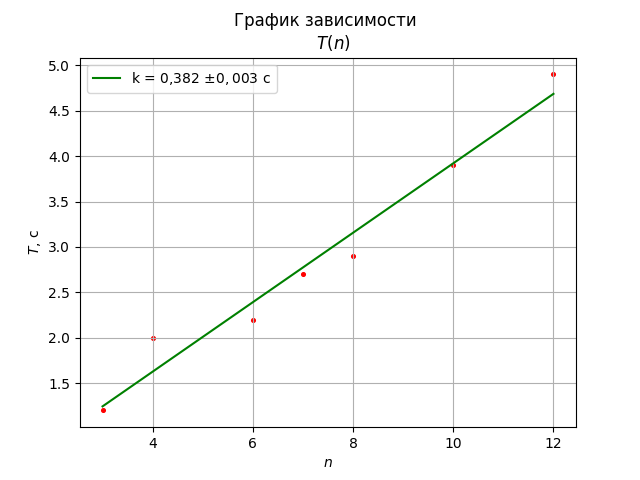
\includegraphics [scale=1]{3-1-3_horizontal.png}}
			\caption{}
		\end{figure}
		\newpage
		\item Построим график зависимости $\mathcal M(n$). По значению углового коэффициента рассчитаем величину вертикальной составляющей магнитного поля Земли.
		
		$$ B_v = \dfrac{ m_{\text{гр}}g r_{\text{гр}}}{\mathfrak m n} = k/\mathfrak m = 0,339 \pm 0,007\text{  Гс}$$
		
		\begin{figure}[H]
			\center{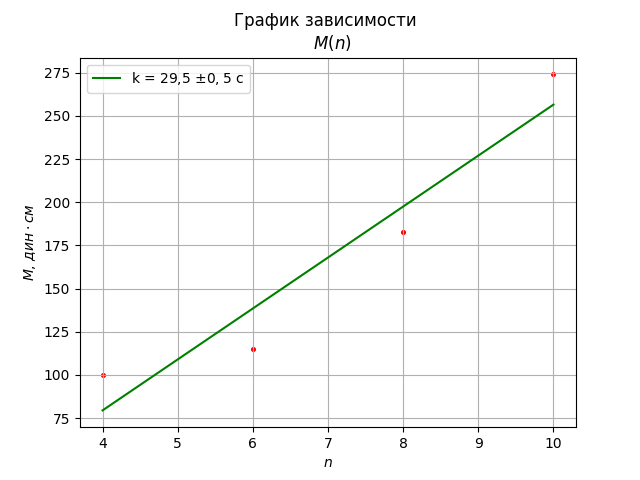
\includegraphics [scale=1]{3-1-3_vertical.png}}
			\caption{}
		\end{figure}
		
		\item Используя результаты измерений $B_h$ и $B_v$, определим магнитное наклонения $\beta$ и полную величину индукции магнитного поля Земли на широте Долгопрудного.
		
		$$ \beta = \arctg \frac{B_v}{B_h} = (75\pm 3) ^{\circ} $$
		$$ B = \sqrt{B_v^2 + B_h^2} = 0,35 \pm 0,01 \text{  Гс}$$
		
		
		\item Проведем эксперимент по измерению зависимости поля B от расстояния r для единичного магнита и набора магнитов. Данные системы можно представить как единичный виток с током и соленоид соответственно. Теория гласит, что зависимость в первом случае будет такая: $B = 2\pi IR^2/(R^2 + r^2)^{3/2} $, где R - радиус витка, во втором случае $B = 2\pi IN/cl \cdot (\cos \beta - \cos \alpha)$, где l - длина соленоида, N - количество витков.
		
		\begin{figure}[H]
			\center{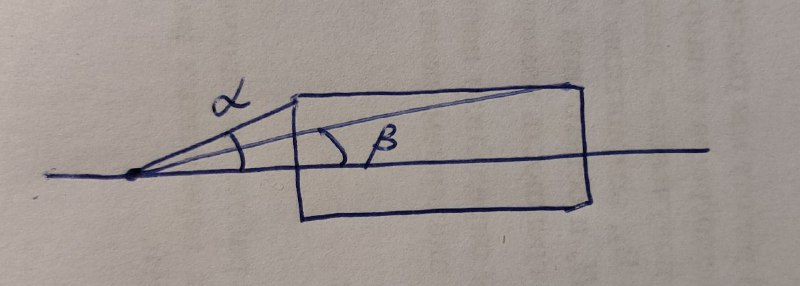
\includegraphics [scale=0.5]{3-1-3_solen.jpeg}}
			\caption{Изображение соленоида для определения углов $\beta, \alpha$ }
		\end{figure}
		
		\begin{figure}[H]
			\center{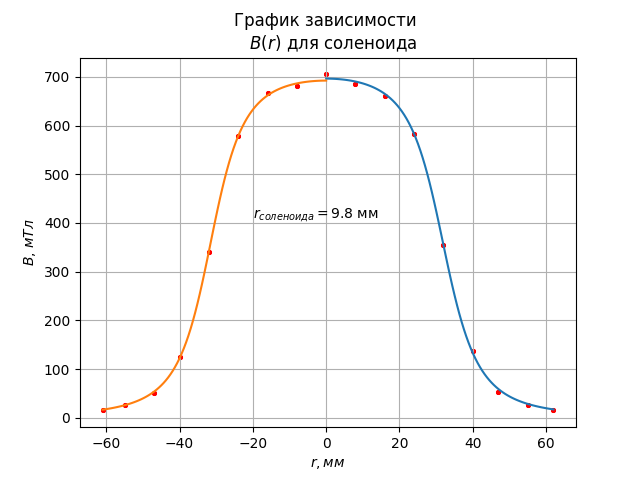
\includegraphics [scale=1]{3-1-3_solenoid.png}}
			\caption{}
		\end{figure}
	
		\begin{figure}[H]
			\center{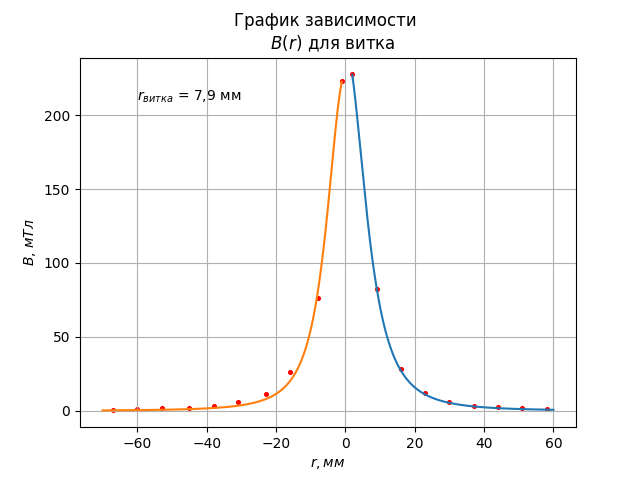
\includegraphics [scale=1]{3-1-3_vitok.png}}
			\caption{}
		\end{figure}
		
	\end{enumerate}
	
	\textbf{Обсуждение результатов и выводы: }\\
	
	В данной работе мы исследовали свойства постоянных неодимовых магнитов,
	измерили с их помощью горизонтальную и вертикальную составляющие
	индукции магнитного поля Земли и магнитное наклонение. Полученные нами результаты немного отличаются от табличных ($B_h = 15$ мкТл, $B_v = 48$ мкТл), это можно объяснить тем, что условия проведения эксперимента не идеальные, так как мы находились в железобетонном здании рядом со множеством металлических изделий, что могли вносить какую-то погрешность. Также мы подтвердили зависимость $B(r)$ для витка с током и соленоида и определили радиус магнитов, из которых состоит соленоид и виток и получили $r_{\text{витка}} = 7.9$ мм и $r_{\text{соленоида}} = 9.8$ мм основной вклад в погрешность вносит погрешность измерения расстояния, полученная относительная погрешность $\varepsilon_r = 3\%$.
	
	
	
	
	
	
	
	
	\end{document}